\chapter{Постановка задачи} \label{chapt2}

Почти все задачи машинного обучения содержат в себе три важные подзадачи:
\begin{enumerate}
    \item Сбор данных
    \item Обучение нейронной сети
    \item Решение инфраструктурных задач
\end{enumerate}

В данном проекте задача решалась итеративно, и цикл повторяется пока решение не будет принято. Причина этому - более экономная трата ресурсов и постоянная обратная связь. Если несколько циклов подряд задачу решить не получается - меняют вводные, либо меняют задачу. 

\section{Содержательная} \label{sect2_1}
\textbf{Дано: } 

Изображение или видеопоток, на котором гарантированно присутствует собака.

\textbf{Требуется: } 

Вернуть информацию о позиции собаки в данный момент на изображении среди следующих классов: [Стоит, сидит, лежит].

Требования к изображению и видеопотоку, которые идут на вход указанной системе. 

Собака в кадре должна быть:
\begin{itemize}
    \item Видна целиком
    \item Ничем не загорожена, даже частично
    \item На кадре находиться одна
    \item Занимать более 50\% кадра по высоте или по ширине
    \item Хвост может быть загорожен телом 
    \item От собаки до края кадра должно быть ещё место, больше 1\% высоты и ширины кадра
 \end{itemize}
 
Камера относительно собаки:
\begin{itemize}
    \item Находится на расстоянии более 2м
    \item Смотрит на собаку на уровне глаз либо выше, но не сверху.
\end{itemize}

Для того чтобы гарантировать присутствие собаки в кадре и тот факт что она одна, будет использоваться другая, отдельная нейронная сеть. 

\section{Математическая}\label{sect2_2}
\subsection{Структура входных данных}
Исходными данными в задаче является конечная последовательность кадров, полученная с видеоряда камеры телефона.

\begin{equation}
    CV = \left\langle
            \begin{matrix}
                I_1 & I_2 & ... & I_3
            \end{matrix}
            \right\rangle
        \end{equation}          

Каждый кадр, или изображение из этого видеоряда является трёхмерной матрицей с количеством столбцов  $h$, количеством строк $w$ и глубиной 3 (красный, зелёный и синий цветовые каналы). 

\begin{equation} 
I =    \begin{bmatrix}
            \begin{bmatrix}
            r_{1,1} & g_{1,1} & b_{1,1}\\
            r_{1,2} & g_{1,2} & b_{1,2}\\
            ...\\
            r_{1,w} & g_{1,w} & b_{1,w}\\
            \end{bmatrix}\\
            \begin{bmatrix}
            r_{2,1} & g_{2,1} & b_{2,1}\\
            r_{2,2} & g_{2,2} & b_{2,2}\\
            ...\\
            r_{2,w} & g_{2,w} & b_{2,w}\\
            \end{bmatrix}\\
            ...\\
            \begin{bmatrix}
            r_{h,1} & g_{h,1} & b_{h,1}\\
            r_{h,2} & g_{h,2} & b_{h,2}\\
            ...\\
            r_{h,w} & g_{h,w} & b_{h,w}\\
            \end{bmatrix}\\
        \end{bmatrix}
\end{equation}

\subsection{Структура выходных данных}\label{input_struct}
В работе требуется построить оператор $F$  который бы заполнял описанную структуру исходя из поставленной задачи:

\begin{equation}
    F:CV \rightarrow RS
\end{equation}

Результаты работы алгоритма заносятся в объект «Состояние собаки»:

\begin{equation}
    RS = \{\begin{matrix}
            prob & loc & breed & pose
        \end{matrix}\}
\end{equation}

,где

$prob$ - число, вероятность того что на кадре присутствует собака.

$loc$ - вектор, содержащий информацию об ограничивающей рамке собаки. Состоит из следующих значений:
\[
loc = \left\langle
            \begin{matrix}
                x_min & x_max & y_min & y_max
            \end{matrix}
\right\rangle
\]

$breed$ - Вектор для вероятностей принадлежности изображения, внутри $loc$ к каждому из 120 классов пород собаки.

$pose$ - Вектор вероятности принадлежности изображения внутри $loc$ к каждой из 3 классов поз собаки.

\subsection{Задача классификации}\label{class_task}
В данной работе решается задача классификации изображений по N классам. 

Классификация\cite{classification} решает следующую задачу.

Задано конечное множество классов и имеется множество объектов, для конечного подмножества которых известно к какому классу они относятся. Это подмножество называется обучающей выборкой. Классовая принадлежность остальных объектов не известна. Требуется построить алгоритм, способный классифицировать произвольный объект из исходного множества.

Классифицировать объект — значит, указать номер (или наименование класса), к которому относится данный объект.

В задачи классификации изображений, объекты — это фотографии. Запишем формальную постановку задачи классификации изображений.

$ CV = 
\left\langle
            \begin{matrix}
                I_1 & I_2 & ... & I_n
            \end{matrix}
\right\rangle
$
~— множество изображений. 
$ Y = 
\{
            \begin{matrix}
                y_1 & y_2 & ... & y_n
            \end{matrix}
\}
$
~— конечное множество меток классов.

$y^{*} : CV \rightarrow Y$ — неизвестная целевая зависимость, значения которой известны только на объектах конечной обучающей выборки 

\[D_m = \{
        \begin{matrix}
            (I_1, y_1) & ... & (I_m, y_m)
        \end{matrix}
    \}
\].

Требуется построить алгоритм $a : CV \rightarrow Y$ , способный классифицировать произвольный объект $I \in CV$.

\subsection{Алгоритм решения поставленной задачи}\label{algorithm}
\begin{figure}[ht] 
  \center
  \includegraphics [width=\textwidth*2/3] {flowchart}
  \caption{Функциональная схема поставленной задачи} 
  \label{img:flowchart}  
\end{figure}
Для того, чтобы гарантировать исполнение условий, указанных в содержательной постановке задачи, используется предобученная нейронная сеть по сегментации изображений MaskRCNN \cite{maskrcnn}, она указана на схеме (рисунок \ref{img:flowchart}) как детектор объектов. Она получает на вход изображение $I$ и возвращает маску объектов $M$, находящихся на ней. 

\[
I \rightarrow M
\]

,где $I$ - Изображение размером 224 пикселя по высоте, 224 пикселя по ширине, обладающее тремя цветовыми каналами $R, G, B$

$M$ - Маска - это бинарное изображение, по высоте и ширине совпадающее с входным изображением, где наличие сигнала (белый цвет) говорит о наличии объекта на кадре. Наглядно это показано на рисунке \ref{img:mask}  .

\begin{figure}[ht] 
  \center
  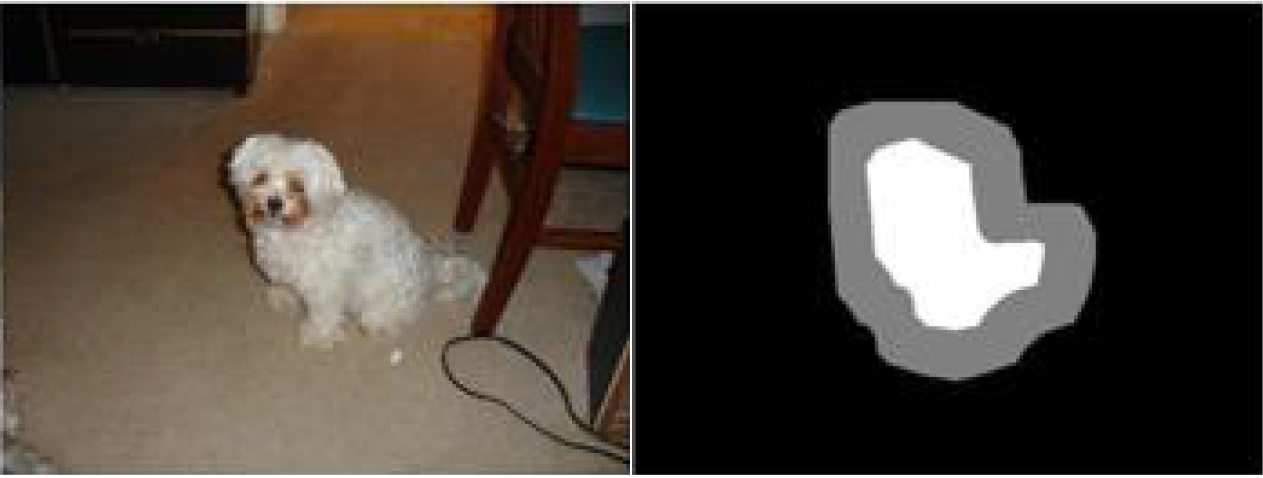
\includegraphics [width=\textwidth] {mask}
  \caption{Изображение собаки и маска собаки для этого изображения} 
  \label{img:mask}  
\end{figure}

Если на маске собаки несколько замкнутых фигур, значит, на кадре больше одной собаки. Если маска собаки пуста, значит на кадре собак нет. Эти две простые проверки сильно увеличивают качество предсказания нейронной сети сети. 

Помимо этих проверок, маска позволяет убрать ненужную часть кадра, уменьшая шанс того, что нейронная сеть ошибётся.

Обрезанное изображение по маске собаки передаётся далее в нейронную сеть для классификации непосредственно позы собаки. На схеме в рисунке \ref{img:flowchart} она указана как классификатор позы собаки. Для этого используется MobileNet v2\cite{mobilenet}. Изменения от оригинальной статьи только в так называемой «голове» классификации и размере входного изображения. Визуально архитектура представлена на рисунке \ref{img:NN_arch} 

\begin{figure}[ht] 
  \center
  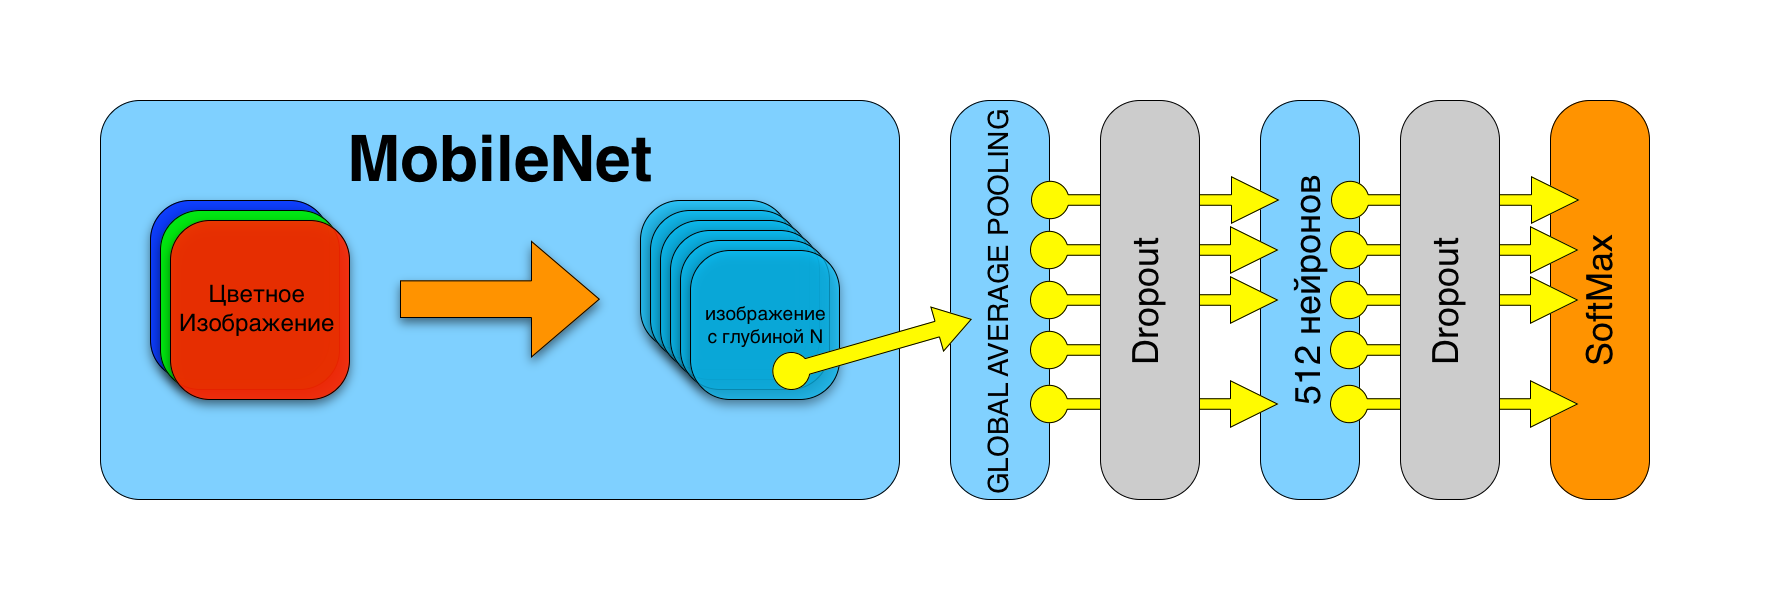
\includegraphics [width=\textwidth] {NN_arch}
  \caption{Архитектура используемой нейронной сети} 
  \label{img:NN_arch}  
\end{figure}

Её характеристики следующие:

\begin{itemize}
    \item Входное изображение I обладает размерностью 96 пикселей по ширине и высоте и 3 цветовыми каналами
    \item Свёрточные слои нейронной сети MobileNet V2\cite{mobilenet}, без "головы".
    \item Global Average Pooling - последняя карта активации(3-мерный тензор $T$ с размерностью $\{x_{d1}, y_{d2}, z_{d3}\}$) преобразуется в плоский вектор $X$ с длинной $d_3$. Каждый слой превращается в одно число - среднее по слою. Это позволяет нейронной сети быть инвариантной к размеру входного изображения.
    
    \[ X_i = \dfrac{1}{d_1*d_2}\sum_{j=0}^{j=d_1}\sum_{k=0}^{k=d_2}T_{i,j,k} \]
    
    \item Слой DropOut\cite{dropout} - обнуление 20\% разных значений предыдущего слоя
    \item Batch Norm\cite{batchnorm} - нормализация вектора относительно других изображений в мини-партии данных для обучения
    \item Полносвязный слой с 512 нейронами
    \item Функция активации, ReLU, см рис \ref{fig:relu}
    
    \[ Relu(x) = max(0,x) \]
    
    
    \begin{figure}
        \centering
        \begin{tikzpicture}[thick,font=\footnotesize]
            \draw[->] (-5,0) -- (5,0) node[right] {Значение на входе};
            \draw[->] (0,0) -- (0,5) node[above] {Значение на выходе};
            \draw[color=blue,domain=-3:0,samples=100] plot (\x,{(0)});
            \draw[color=blue,domain=0:4,samples=100] plot (\x,{(\x)});
        \end{tikzpicture}
        \caption{График функции активации ReLU}
        \label{fig:relu}
    \end{figure}
    
    \item DropOut
    \item BatchNorm
    \item Выходной слой $n$ нейронов, по количеству классов. Функция активации softmax. 
    \[softmax(x)_i = \frac{exp(x_i)}{\sum_{j}^{ }exp(x_j))}\]
\end{itemize}

Такая архитектура обусловлена борьбой с переобучением нейронной сети на маленьких объёмах данных. Размер входного изображения держался на минимальном уровне: в то время, как обычно нейронные сети используют по 224 пикселя по длине и 224 ширине, здесь же всего 96. 

Множественные DropOut и Batch Normalization тоже сильно мешают нейронной сети "зазубрить" датасет, так как они каждый раз немного изменяют выходы предыдущих слоёв. Сама архитектура MobileNet тоже выбрана не случайно. Она обладает крайне малым количеством обучаемых параметров, при этом выдаёт совершенно замечательные результаты классификации известных датасетов.\cite{mobilenet} Это можно видеть на рисунке \ref{img:resnet}.

\begin{figure}[ht] 
  \center
  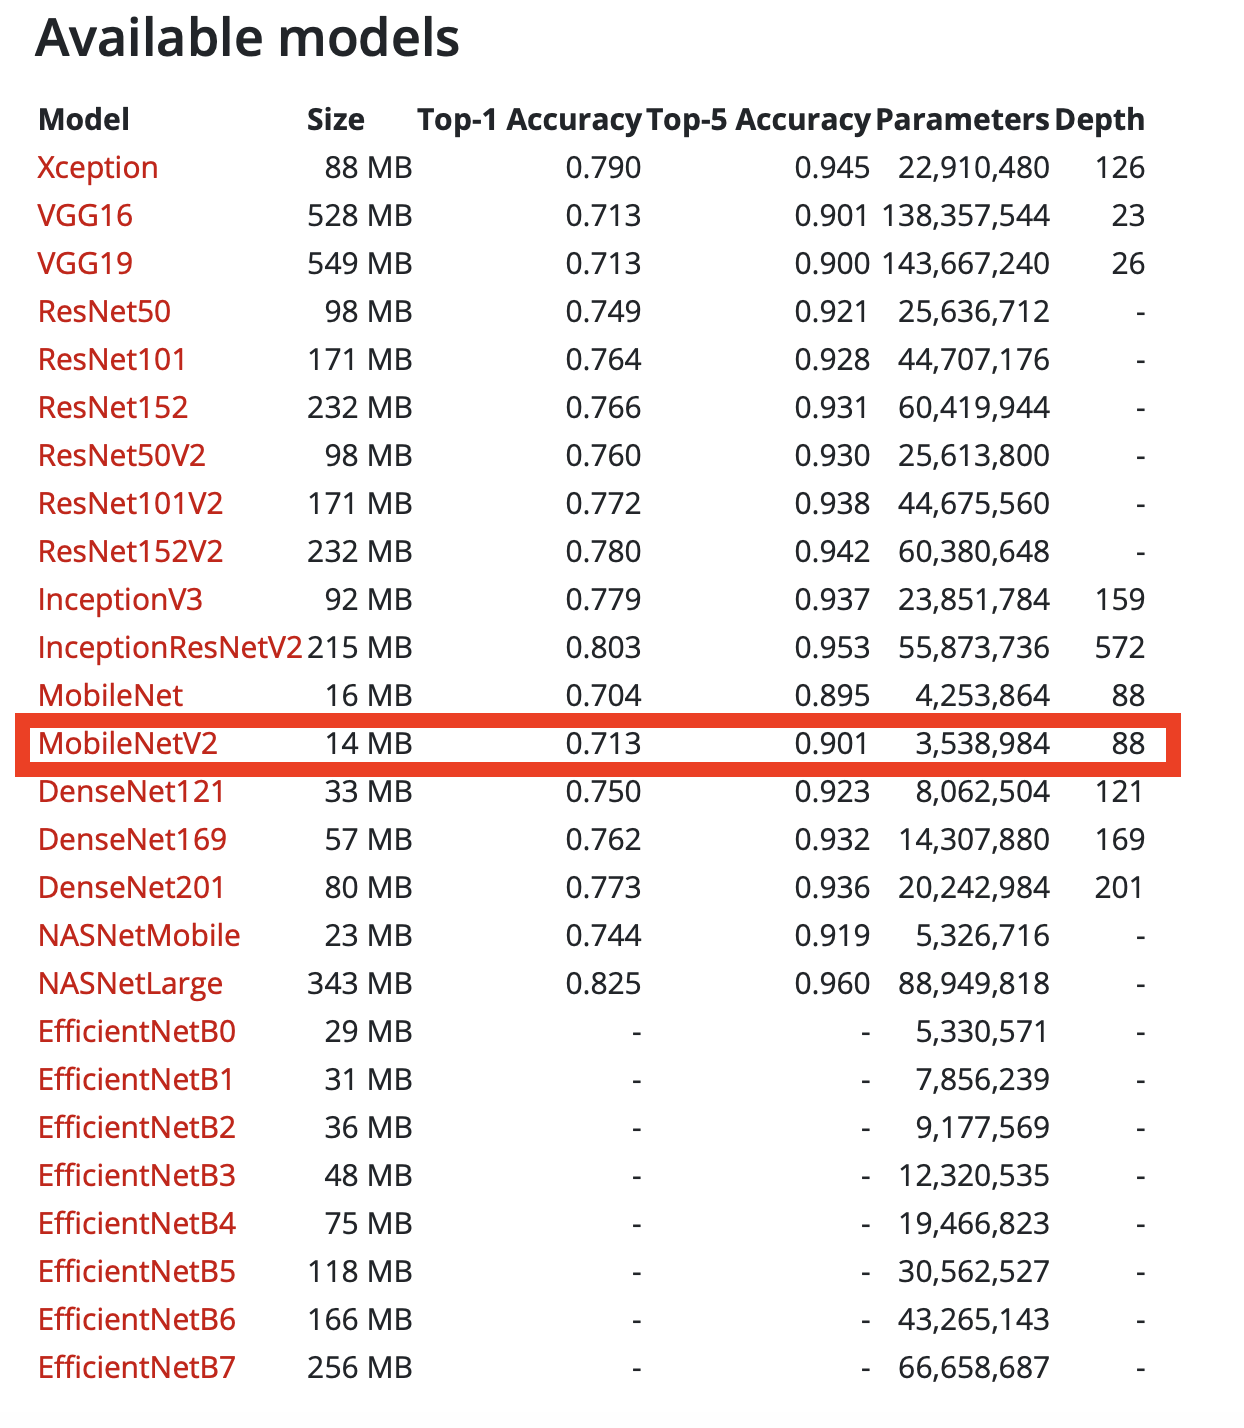
\includegraphics [width=\textwidth*2/3] {mobilenet_vs_rest}
  \caption{MobileNet обладает практически минимальным количеством обучаемых параметров, при этом не отстаёт по точности от других архитектур} 
  \label{img:resnet}  
\end{figure}


\subsection{Инструменты и средства разработки}\label{ide}
Программное обеспечение алгоритма распознавания позы собакибыл реализовано на языке программирование Python с помощью библиотеки компьютерного зрения OpenCV, а также библиотеки для обучения нейронных сетей Keras в интегрированной среде разработки PyCharm.

Python - интерпретируемый язык с динамической типизацией общего назначения. Данный язык программирования поддерживает такие парадигмы программирования, как процедурное программирование, объектно-ориентированное программирование и обобщенное программирование. Также он обеспечивает модульность, обработку исключений, трассировку ошибок, абстракцию данных, объявление классов объектов и лямбда-функции.

OpenCV (англ. Open Source Computer Vision Library, библиотека компьютерного зрения с открытым исходным кодом) — библиотека алгоритмов компьютерного зрения, обработки изображений и численных алгоритмов общего назначения с открытым кодом.

Приложение для мобильного телефона разрабатывалось в интегрированной среде разработки XCode с применением библиотек Metal, CoreML и Vision. CoreML является библиотекой для машинного обучения и работы с нейронными сетями для продуктов компании Apple и сделан на базе Metal, который позволяет использовать специализированные инструкции новых процессоров включая Neural Engine, который ускоряет работу с нейронными сетями в несколько раз. В качестве языка для приложения на телефоне использовался Swift 4.2. 